%Corps du document :
%\setlength{\parindent}{1cm}    

\section{Introduction}

Ce projet de système d'information urbanisé nous a permis, au cours de ces quatre séances, de nous familiariser avec la conception d'un système applicatif orienté objet complexe. Il nous a également permis de mettre en application la méthode de conception vue en cours, ainsi que de compléter notre expérience personnelle en matière de systèmes d'information.

\section{Distribution des charges}

\begin {center}
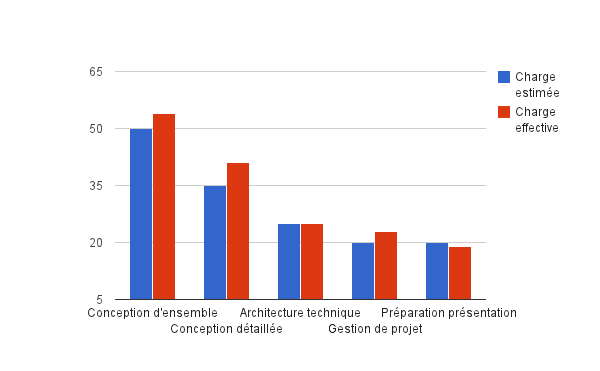
\includegraphics[width=\textwidth]{charges-effectives.png}
\end {center}

Dans l'ensemble, les charges ont été équitablement distribuées. Les temps évalués pour chacune de ces tâches ont dans l'ensemble été respectés, même si quelques temps ont été légèrement sous- ou surestimés. La charge totale estimée était cohérente, et cette bonne évaluation des temps nous a permis de travailler avec un rythme soutenu et efficace.

En revanche, certaines dépendances bloquantes entre des tâche ont provoqué des goulots d'étranglement ; ce fut le cas, en particulier, de la succession des diagrammes d'activité, de séquence, et de collaboration. Pour pallier à ce problème, nous avons parallélisé le travail entre plusieurs personnes qui formaient un groupe de travail commun. Ces personnes construisaient chacun leur diagramme de leur côté, et communiquaient leurs choix régulièrement pour harmoniser leur travail avec celui des autres.

\section{Appropriation des méthodes}

Notre équipe a globalement bien assimilé et intégré la méthode de conception Système d'Information urbanisé. L'approche que nous avons adoptée était cohérente, bien qu'elle aurait bénéficié à être plus orienté métier. En effet, on dénote souvent dans les livrables et diagrammes un aspect développement et implémentation assez fort, parfois au détriment de l'aspect métier. Nous sommes donc paré pour les futurs projets SI que nous rencontrerons, à l'INSA ou dans notre vie professionnelle, et nous saurons accorder toute son importance au \textbf{métier}.

\section{Une communication efficace}

La communication entre les membres de l'équipe a été grandement facilitée et accélérée par un usage extensif des dernières technologies du web. En effet, nous avons fait usage d'outils de rédaction collaborative de documents tels que Google Docs, des outils de gestionnement tel que GitHub, des outils de communication et d'échange en temps réel. Travailler collaborativement à plusieurs sur l'établissement d'un diagramme est une expérience formidable et permet d'éliminer les risques d'incompréhension et de mauvaise communication. De surcroît, cela garantie l'harmonisation des différentes étapes du projet.

Parmi les outils utilisés, nous pouvons citer Cacoo.com, programme de création de graphes, websequencediagrams.com, logiciel de création de diagrammes de séquence, ou encore typewith.me, éditeur de texte collaboratif, sans compter le nombre de sites d'information et de question-réponses qui ont fait mûrir nos réflexions.

\section{Conclusion}

Ce projet dans son ensemble a été pour nous une expérience enrichissante et constructive. Il nous a permi de nous faire la main sur un projet de Système d'Information Urbanisé et SOA concret, de mettre en place des méthodes de travail productives et efficaces, et nous avons maintenant toutes les clefs en main pour une carrière d'ingénieur SI solide et un futur prometteur.
